%\documentclass{jpsj3}
\documentclass[fp,twocolumn]{jpsj3}
%\documentclass[letter,twocolumn]{jpsj3}
%\documentclass[letterpaper,twocolumn]{jpsj3}
\usepackage{txfonts}
\usepackage{algorithm}
\usepackage{algorithmic}
\usepackage{amsmath}
\usepackage{multirow}

\makeatletter
\@dblfptop 0pt
\makeatother

\renewcommand{\topfraction}{.85}
\renewcommand{\bottomfraction}{.60}
\renewcommand{\textfraction}{.15}
\renewcommand{\floatpagefraction}{.6}

\title{Derivaton of the QUBO formulation for sparse estimation}

\author{Tomohiro Yokota$^1$%\thanks{jpsj{\_}edit@jps.or.jp}
  , Jun Ohkubo$^1$, Makiko Konoshima$^2$, Hirotaka Tamura$^2$}
\inst{$^1$Graduate School of Science and Enginnering, Saitama University,
  255 Shimo-Okubo, Sakura-ku, Saitama-shi, 338-8570, Japan\\
$^2$Fujitsu Laboratories Ltd.,
4-1-1 Kawasaki, Kanagawa 211-8558, Japan} %\\

\abst{In recent years, annealing machine have been developed, and their use methods are considered in fields such as optimization problems and machine learning. In the annealing machine, it is necessary to express the problem to be dealt with in QUBO(Quadratic Unconstrained Binary Optimization) formulation and implement it as hardware. However, since the general method of rewriting to the QUBO format is not known yet, it needs to be derived individually. In this paper, we derive the QUBO formulation for the l1-norm (absolute value function) used in sparse estimation. As a result of experiment, it was possible to predict that one variable could be reduced from the result of numerical experiment by applying the Legendre transformation and Wolf-duality theorem to l1norm. By reviewing the formulation we were actually able to reduce one variable.

l1-normのQUBO形式での定式化を提案する. これにより, スパース推定に対するQUBO形式を導出することができるようになる. Sato et al.(2019)が提案したReLUタイプ関数の定式化の方法を応用することで, l1-normのQUBO形式での導出を行なった. 加えて, 数値実験を通して, 定式を見直すことにより変数を減らすことができた. 
}

%%% Keywords are not needed any longer. %%%
%%% \kword{keyword1, keyword2, keyword3, \1dots} 
%%%

\begin{document}
\maketitle

\section{Introduction}
In recent yeaars, sepecial machines for annealing have benn developed such as D-Wave Systems Inc.'s D-Wave\cite{d-wave01, d-wave02} and Fujitsu's Digital Annealer\cite{DA} and methods for use in various fields are being considered. The annealing machine acceptes Ising model parameters as input, but there are many functions thathave been represented yet because systematic derivation of the Ising model has been shown.
In the previous researches, the robust q-loss function is derived in the QUBO form using the Legendre transform\cite{q-loss}, and its performance is evaluated using the classification problem as an example. Also, in the recently published papaer on the derivation of the ReLU function in the QUBO form\cite{relu}, the derivation has made using the Wolfe-duality theorem\cite{wolfe}, so that the Legendre transformation alone is insufficient.
On the other hand, sparse estimation is used in the fields of image processing and machine learning, and it is an important research in reducing the number of data, selecting related data from high-dimensional and complex data and making it simple.
The purpose of this research is to derive an l1-norm, which is a regularization term of Lasso\cite{lasso} used in sparse estimation, in the QUBO form using the derivation method in \cite{relu}. Furthemore, we evaluate whether the derived result is correct using simulated anneaing.

近年では, D-Wave Systems Inc.のD-Waveや富士通のデジタルアニーラのようなイジング型マシンの開発が進められている. 利用できる量子ビット数が年々増加しており, これにより大きな組み合わせ最適化問題に対してイジング型マシンでの計算ができるようになった. しかし, イジング型マシンで最適化問題を計算するためには, コスト関数をQUBO形式に変換しハードウェアとして実装する必要があるが, その系統的な導出方法はまだ見つかっていない. 

先行研究ではq-loss関数とReLUタイプ関数のQUBO形式での導出がされている. q-loss関数の導出法についてはLegendre変換を適用することでQUBO形式を導出することができた. しかし, ReLUタイプ関数に対しては, q-loss関数の導出法と同様にLegendre変換だけを適用した場合, コスト関数のmin関数にマイナス符号がついてしまっている. これによりReLUタイプ関数を他のコスト関数を組み合わせた最適化問題を解くことが困難になる. そこで, Wolfeの双対定理を適用した. 

本稿で紹介するl1-normはスパース推定を行う際に利用されている. スパース推定はデータ解析や画像処理の分野で利用されている. データ解析ではスパース推定を用いることで解がスパースになる. この考え方は, ブラックホールの解析でも利用されている. ブラックホールとても小さく, 今までの手法では解像度が低いため観測することが不可能であった. そこで, 世界中の電波望遠鏡から同時に測定を行い, その観測データに対してスパース推定を行うことで本質的な情報のみを取り出しブラックホールの画像化を行なった. ここで, l1-normのQUBO形式での導出はまだされておらず, イジング型マシンを用いたスパース推定を行う上でこの研究は重要である.

本稿ではl1-normのQUBO形式での定式化を行う. そのために, Legendre変換およびWolfeの双対定理を用いる. さらに, 定式化を見直すことで, 単純に適用した場合よりも変数を減らせることが確認できた. これはイジング型マシンの量子ビット数に制限がある現在において, ハードウェアへの実装を考える上で重要なことである. 

構成について

\section{Background}
In this section, we describes the knowledge and algorithms used in the exeriment.

\subsection{QUBO and Ising model} %QUBOとIsingモデルについての説明
Since the QUBO formulation and the Ising model are equivalent, we can be converted to other form if we can be represented one side. The Ising model is represented as follows:
\begin{eqnarray}
  H=-\sum_{i,j}{J_{i,j}\sigma_{i}\sigma_{j}}-\sum_{i}{h_{i}\sigma_{i}}
\end{eqnarray}
where $\sigma_{i}\in \{-1,+1\}$is a spin variable for $i$-th spin, $J_{ij}\in \mathbb{R}$ a quadratic term of $i$ and $j$, and $h_{i}\in \mathbb{R}$ a liner term of $i$. We can easily converted the Ising model to QUBO formulation, which uses binary variable $q_{i}\in \{0,1\}$, by applying $q_{i}=\frac{\sigma_{i}+1}{2}$ and QUBO formulation is represented as follows:
\begin{eqnarray}
  H=-\sum_{i,j}{\tilde{J}_{i,j}q_{i}q_{j}}-\sum_{i}{\tilde{h}_{i}\sigma_{i}}
\end{eqnarray}

\subsection{}

\subsection{Simulated Annealing} %実験で利用するSAアルゴリズムについての説明
Simulated annealing(SA) is optimization algorithm, and it find the minimum of the objective function efficiently. SA repeatedly minimize the objective function by moving the variables randmoly (in this papaer, it moves at a fixed size) at each iteration. Also, it does not necessarily reject non-minimizing movement, but accepts it with a certain acceptance probability. It is possible to avoid convergence to the local minimum. Here, the acceptance probability is inversely proportional to the inverse temperature (execution time) and the size of the energy difference before and after movement. Algorithm.\ref{alg:SA} show the SA algorithm. We uses the temperature function $T(n+1)=\alpha T(n) (0<\alpha <1)$ and run the SA algorithm until the temperature becomes small.

%シミュレーテッドアルゴリズムの図
\begin{algorithm}
  \caption{Simulated Annealing}
  \begin{algorithmic}[1]
    \REQUIRE variables $m, t, z_{1}, z_{2}$, initila temperature $T_{0}$, lower limit temperature $T_{limit}$, initial random state with $-10\leq m\leq 10, -1\leq t\leq 1, 0\leq z_{1}\leq 10$ and $0\leq z_{2}\leq 10$ 
    \ENSURE  $t, z_{1}, z_{2}$ of local minimum when $m$ is given.
    \FOR{$n\leftarrow 1$ to $T(n)<T_{limite}$}
    \STATE Evaluate the cost $L(m, t, z_{1}, z_{2})$ at the current state
    \STATE Let $t', z_{1}'$ and $z_{2}'$ be random move of $t,z_{1}$ and $z_{2}$ and evaluate the cost $L(m,t',z_{1}', z_{2}')$
    \STATE $\Delta \leftarrow L(m,t',z_{1}',z_{2}') - L(m,t,z_{1},z_{2})$
    \STATE $p\leftarrow \exp{(\Delta /T(count))}$
    \STATE Update $t,z_{1},z_{2}$ to $t',z_{1}',z_{2}'$with probability $\min{(1,p)}$, otherwise do not update
    \ENDFOR
  \end{algorithmic}
  \label{alg:SA}
\end{algorithm}

\subsection{Lasso}
Lasso(Least Absolute Shrinkage and Selection Operator) is a method to estimate regression coefficients sparsely by using l1-norm regularization terms. The cost function of Lasso is represented as follows:
\begin{eqnarray}
  \frac{1}{2n}*\|y-Xw\|^{2}_{2} + \alpha\|w\|_{1}
\end{eqnarray}
where $ $. Here, since the Lasso regularization term is not continuous, updating by partial differentation with respect to parameter $\alpha$ can not be obtain. So, in the next section, we will explain how to obtain the update formula of $alpha$ using the Coordinate Descent.

\subsubsection{Coordinate descent}
Coordinate Descent is an algorithm, which updates by repeating the procedure of fixing the values of $p-1$ elements among $p$ parameters and updating only one remaining parameter for all elements.

\section{Derivation of l1-norm in QUBO formulation} %l1-normのQUBOでの定式化
We define the function $f(m)$ as follows:
\begin{eqnarray}
  f(m)=-\min{(-m,m)}
\end{eqnarray}
\begin{figure}[htbp]
  \begin{center}
    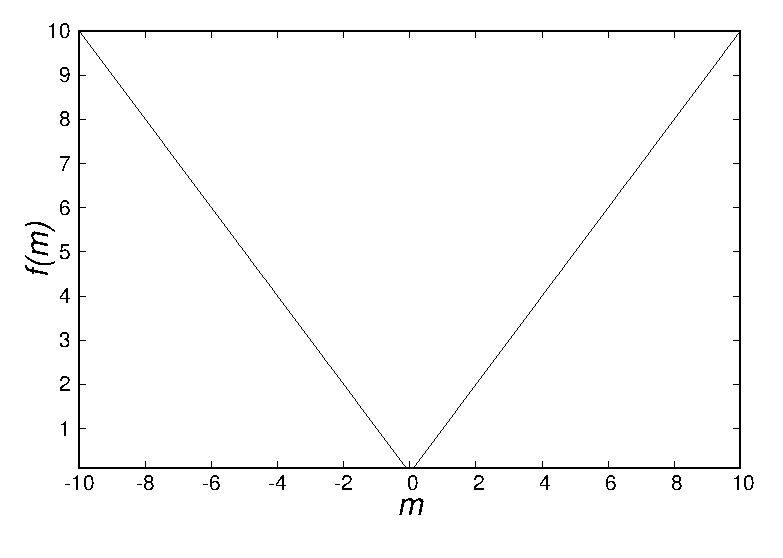
\includegraphics[keepaspectratio,scale=0.50]{absolute.eps}
    \caption{Outline of l1-norm}
    \label{fig:absolute}
  \end{center}
\end{figure}
A function form of $f(m)$ is shown in Fig.\ref{fig:absolute}. We convert $f(m)$ to quadratic form by applying the Legendre transform to it. Using the method used in the papaer, the one converted to quadratic form is represented as follows:
\begin{eqnarray}
  F(m)=-\min_{t}{\{-mt\}} \quad \text{subject to} \quad \-1 \leq t \leq 1 \label{legendre}
\end{eqnarray}
We could express the quadratic form of $f(m)$ as (\ref{legendre}), but there is the min function is proceded by a minus sign, which makes it difficult to solve an optimization problem that combines multiple cost functions. Let the other cost function be $C(m)$, and the combination with $F(m)$ is as follows:
\begin{eqnarray}
  \min_{m}{\{C(m)+F(m)\}} &=& \min_{m}\left\{C(m)-\min_{t}{\{-mt\}}\right\} \nonumber \\
  &\neq & \min_{m,t}{\left\{C(m)-(-mt)\right\}} \nonumber 
\end{eqnarray}
Hence, it is not in the form of minimization problem for both $m$ and $t$.
In precious researche \cite{relu}, this problem was solved by applying Wolfe dual theorem to (\ref{legendre}). By applying this theorem, the dual problem of the optimization problem (\ref{legendre}) is represented as follows:
\begin{eqnarray}
  F'(m)=\max_{t,z_{1},z_{2}}{\{-mt-z_{1}(t+1)+z_{2}(t-1)} \label{wolf}
\end{eqnarray}
\begin{equation}
  \text{subject to} \quad \left\{
  \begin{aligned}
   -m-z_{1}&+z_{2}=0, \nonumber \\
   \ -1\leq t\leq 1,& z_{1}\geq 0, z_{2}\geq 0 \nonumber \\
  \end{aligned}
  \right.
\end{equation}
In order to remove the equality constraint ($-m-z_{1}+z_{2}=0$), it is enough to add the following penalty term of the square of it. Therefore, the optimization problem (\ref{wolf}) can be represented as follows:
\begin{equation}
  \begin{aligned}
    F'(m)&=\min_{t,z_{1},z_{2}}{\{mt+z_{1}(t+1)-z_{2}(t-1)} \\
    &\quad+M(-m-z_{1}+z_{2})^{2}\} \label{after_wolf} \\
  \end{aligned}
\end{equation}
\begin{eqnarray}
  \text{subject to} \quad -1\leq t\leq 1, z_{1}\geq 0, z_{2}\geq 0 \nonumber
  \end{eqnarray}
where M is a constant and take a large value to ensure the equality constraint ($-m-z_{1}+z_{2}=0$) to be satisfied, and the remaining inequality consraints conditions ($-1\leq t\leq 1, z_{1}\geq 0$ and $z_{2}\geq 0$) can be easily realized by expanding these variables $t,z_{1}$ and $z_{2}$, in the binary expressions which satisfy the corresponding domain constraints. We will varify in the next section that the (\ref{after_wolf}) is correctly fomulated. 

\subsection{Results} \label{experiment_condition} %定式化したものを利用して実験を行う
In this section, we verify that the formulation is correct by optimizing problem (\ref{after_wolf}) with SA Algorithm. \ref{alg:SA}. Each variable moves by +0.001 or -0.001 with the same probability for each iteration. The 10,000 times execution results when $T(0)=1000$, $\alpha=0.9999$ and running algorithm until $T(n)<0.001$ are as shown in the Fig.\ref{fig:minimum1}.

\begin{figure}[htbp]
  \begin{center}
    \begin{tabular}{c}
      \begin{minipage}{0.50\hsize}
        \centering
        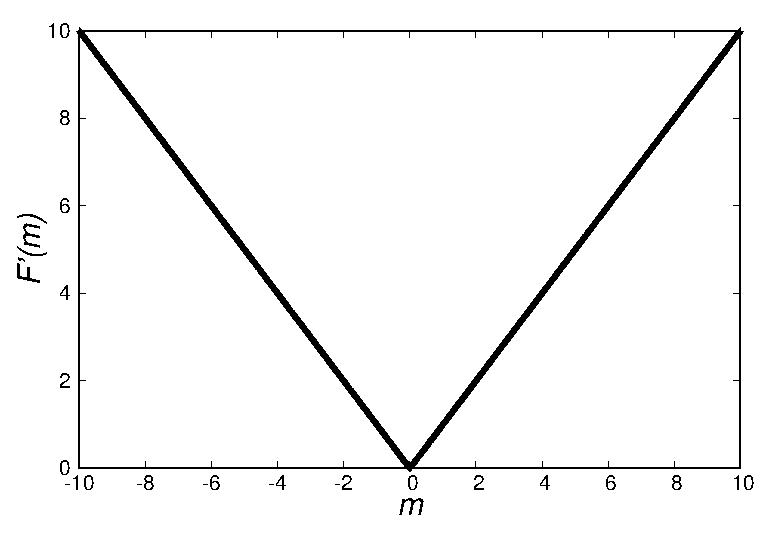
\includegraphics[keepaspectratio,scale=0.33]{minimum_cost.eps}
      \end{minipage}
      \begin{minipage}{0.50\hsize}
        \centering
        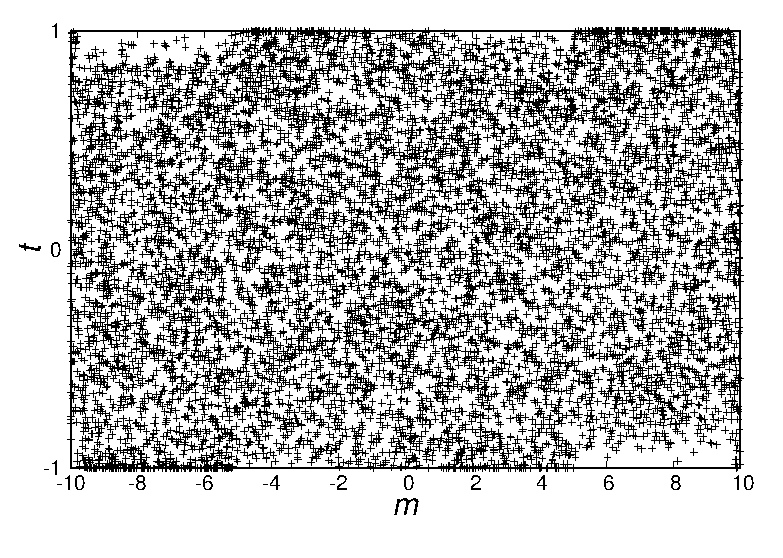
\includegraphics[keepaspectratio,scale=0.33]{minimum_t.eps}
      \end{minipage} \\
      \begin{minipage}{0.50\hsize}
        \centering
        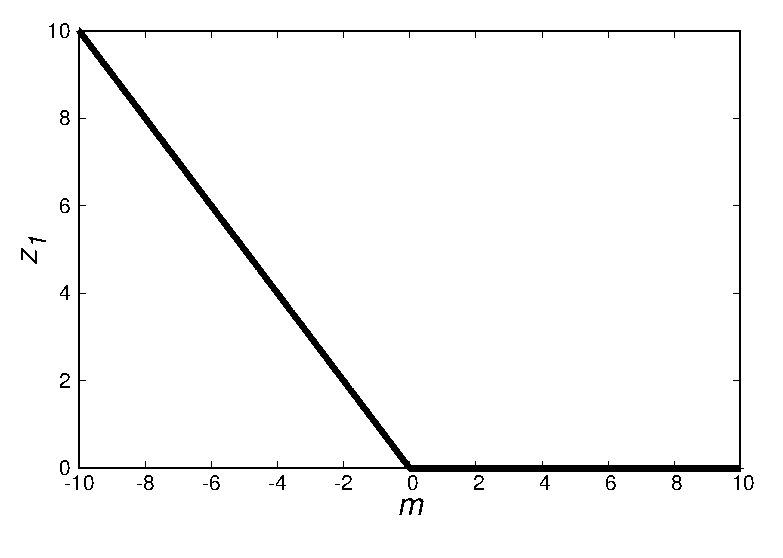
\includegraphics[keepaspectratio,scale=0.33]{minimum_z1.eps}
      \end{minipage}
      \begin{minipage}{0.50\hsize}
        \centering
        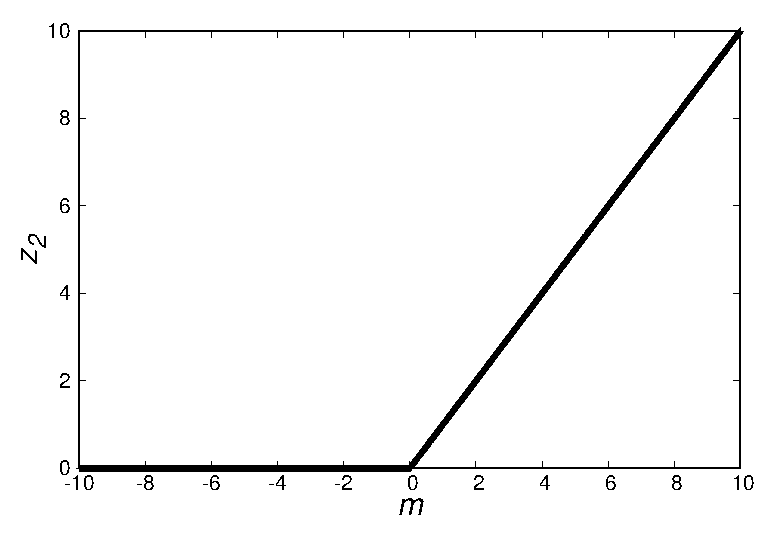
\includegraphics[keepaspectratio,scale=0.33]{minimum_z2.eps}
      \end{minipage}
    \end{tabular}
    \caption{The figures for upper left, upper right, lower left and lower right show the results when $F'(m), t, z_{1}, z_{2}$ are optimized for each $m$ respectively.}
    \label{fig:minimum1}
  \end{center}
\end{figure}
From this result, we can confirm that l1-norm can be obtained by optimizing (\ref{after_wolf}). Also, if we look at each variable $t, z_{1}$ and $z_{2}$ at optimization, we can see the following: It may be possible to reduce one variable by reviewing the (\ref{after_wolf}) because $t$ is not converged alothough $z_{1}$ and $z_{2}$ converge to a specific value.

\section{Reviewing formulation} %定式化の見直し
We can think of the following from the results of the numerical experiments in the previous section: The variable $t$ seems to be taking a random value rather than settling to the optimal value, so we will consider whether we can eliminate $t$ by reviewing the formulation. 
The cost function can be transformed as follows using equality constraint.
\begin{alignat}{2}
  F'(m)&=\min_{t,z_{1},z_{2}}{\{mt+z_{1}(t+1)-z_{2}(t-1)} \nonumber \\
  &\quad+M(-m-z_{1}+z_{2})^{2}\} \nonumber \\
  &=\min_{t,z_{1},z_{2}}{\{mt+z_{1}(t+1)-(m+z_{1})(t-1)} \nonumber \\
  &\quad+M(-m-z_{1}+z_{2})^{2}\} \nonumber \\
  &=\min_{z_{1},z_{2}}{\{z_{1}+(m+z_{1})+M(-m-z_{1}+z_{2})^{2}\}} \nonumber \\
  &=\min_{z_{1},z_{2}}{\{z_{1}+z_{2}+M(-m-z_{1}+z_{2})^{2}\}} \label{review_formulation}
\end{alignat}
This conversion from (\ref{after_wolf}) to (\ref{review_formulation}) is possible because the penalty term, $M(-m-z_{1}+z_{2})^{2}$, forces the equality constraint to be satisfied.

\subsection{Results} %定式化したものを利用して実験を行う
The result of experimenting the optimization problem under the same experimental conditions as Section\ref{experiment_condition} with (\ref{review_formulation}) as the objective function is as shown in Fig.\ref{fig:minimum2}.
\begin{figure}[htbp]
  \begin{center}
    \begin{tabular}{c}
      \begin{minipage}{0.50\hsize}
        \centering
        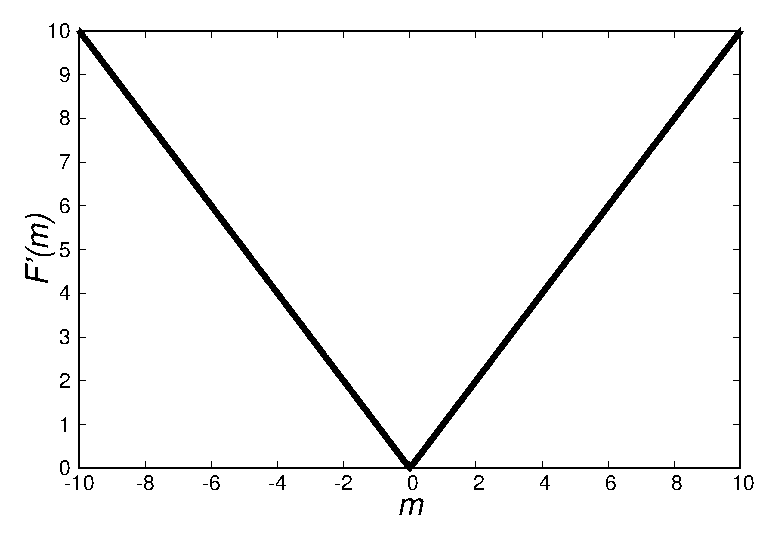
\includegraphics[keepaspectratio,scale=0.33]{minimum_cost_non_t.eps}
      \end{minipage} \\
      \begin{minipage}{0.50\hsize}
        \centering
        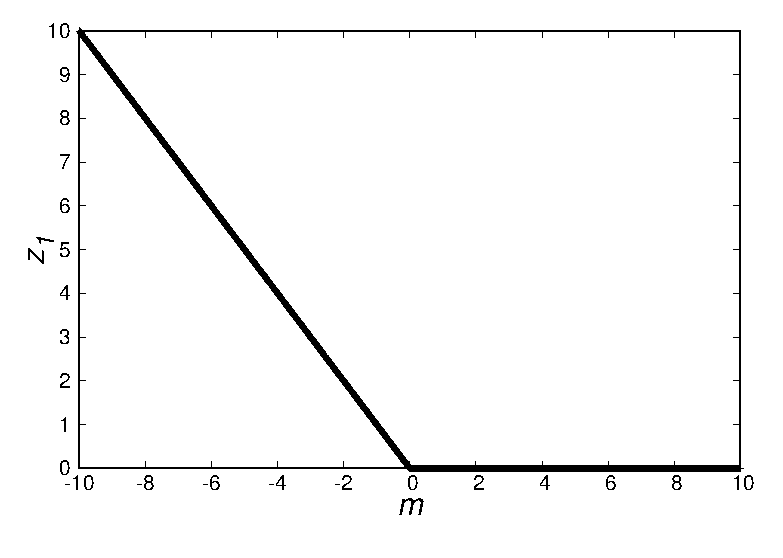
\includegraphics[keepaspectratio,scale=0.33]{minimum_z1_non_t.eps}
      \end{minipage}
      \begin{minipage}{0.50\hsize}
        \centering
        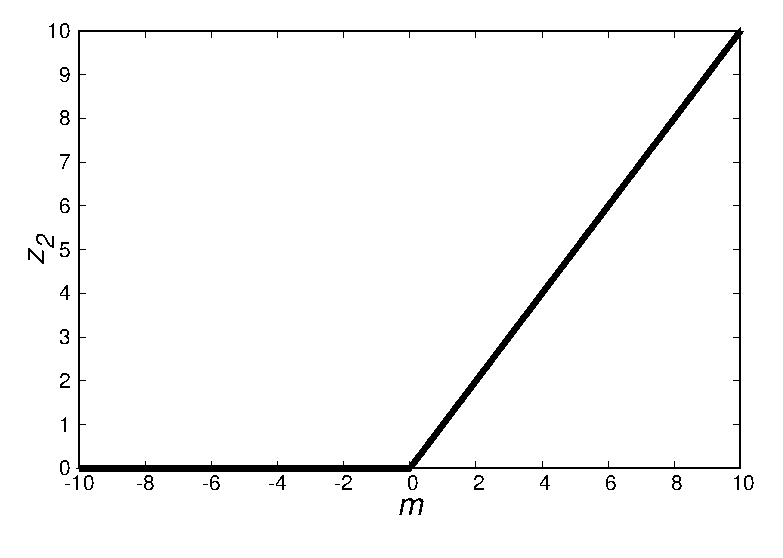
\includegraphics[keepaspectratio,scale=0.33]{minimum_z2_non_t.eps}
      \end{minipage}
    \end{tabular}
    \caption{The figures for upper, lower left and lower right show the results when $F'(m), z_{1}, z_{2}$ are optimized for each $m$ respectively.}
    \label{fig:minimum2}
  \end{center}
\end{figure}
From this result, the outline of $F'(m), z_{1}$ and $z_{2}$ when optimizing (\ref{after_wolf}) did not change from Fig.\ref{fig:minimum2}, so we seem that removing the variable $t$ does not affect the result.

\section{Comparetive experiment} %Lasso について比較実験を行う ここではアニーリングとpythonのskite-learnのLassoで比較実験を行う データはBosoton.csvを使用
% アニーリングでのパラメータの設定についてとpythonの設定を記述する

\subsection{Results}
\begin{table}
  \begin{tabular}{|c||r|r|} \hline
    elements  & Coordinate Descent & Annealing \\ \hline
    "crim"    & -0.00000000 & -0.015 \\
    "zn"      &  0.00000000 &  0.000 \\
    "indus"   & -0.00000000 & -0.002 \\
    "chas"    &  0.00000000 &  0.014 \\
    "nox"     & -0.00000000 & -0.002 \\
    "rm"      &  2.71542789 &  2.829 \\
    "age"     & -0.00000000 &  0.000 \\
    "dis"     & -0.00000000 & -0.000 \\
    "rad"     & -0.00000000 & -0.000 \\
    "tax"     & -0.00000000 & -0.013 \\
    "ptratio" & -1.34428304 & -1.305 \\
    "black"   &  0.18036988 &  0.234 \\
    "lstat"   & -3.54677609 & -3.456 \\ \hline
  \end{tabular}
\end{table}

\begin{acknowledgment}

%\acknowledgment

%For enveironments for acknowledgment(s) are available: \verb|acknowledgment|, \verb|acknowledgments|, \verb|acknowledgment|, and \verb|acknowledgments|.

\end{acknowledgment}

%\appndix
%\section{}
%Use the \verb|\appendix| command if you need an appendix(es). The \verb|\section| command should follow even though there is no title for the appendix (see above in the source of this file).
%For authurs of Invited Review Papers, the \verb|profile| command si prepared for the author(s)' profile. A simple example is shown below.

%\begin{verbatim}
%\profile{Taro Butsuri}{was born in Tokyo, Japan in 1965. ...}
%\end{verbatim}

\begin{thebibliography}{1}
\bibitem{d-wave01}
  M. W. Johnson, M. H. S. Amin, S. Gildert, T. Lanting, F. Hamze, N. Dickson, R. Harris, A. J. Berkley, J. Johansson, P. Bunyk, E. M. Chapple, C. Enderud, J. P. Hilton, K. Karimi, E. Ladizinsky, N. Ladizinsky, T. Oh, I. Perminov, C. Rich, M. C. Thom, E. Tolkacheva, C. J. S. Truncik, S. Uchaikin, J. Wang, B. Wilson and G. Rose, Nature. {\bf 473}, 194 (2011).
\bibitem{d-wave02}
  P. I. Bunyk, E. Hoskinson, M. W. Johnson, E. Tolkacheva, F. Altomare, A. J. Berkley, R. Harris, J. P. Hilton, T. Lanting, J. Whittaker, IEEE Trans. Appl. Supercond. {\bf 24}, 1700110 (2014).
\bibitem{DA}
  M. Aramon, G. Rosenberg, E. Valiante, T. Miyazawa, H. Tamura, and H. G. Katzgraber, arXiv:1806.08815.
\bibitem{q-loss}
  V. Denchev, N.Ding, S. V. N Vishwanathan, and H. Neven, in Proceedings of the 29th International Conference on Machine Learning, p.863 (2012).
\bibitem{relu}
  Go Sato, Makiko Konoshima, Takuya Ohwa, Hirotaka Tamura and Jun Ohkubo, arXiv:1911.03829.
\bibitem{wolfe}
  P. Wolfe, Quart. Appl. Math. {\bf 19}, 239 (1961).
\bibitem{lasso}
  Robert Tibshirani, Regression Shrinkage and Selection via the Lasso, J. R. Statist. Soc, B, 58(1):267-288 (1996).
  
\end{thebibliography}

\end{document}


